%\documentclass[a4paper,english,12pt,twocolumn]{article}
\documentclass[a4paper,english,12pt]{article}
\usepackage[utf8]{inputenc} % Encodage du fichier
\usepackage[T1]{fontenc} % Encodage des fonts nécessaire pour le Latin
\usepackage[french]{babel} % Pour changer la langue des mots générés et choisir la bonne mise en page
\usepackage{amssymb}
\usepackage{pdflscape}
\usepackage{microtype} 
\usepackage{lmodern} % Le latin modèrne
\usepackage[top=2cm, bottom=2cm, left=2.5cm, right=1.5cm]{geometry} % Définir les marges de la page 
\usepackage[hidelinks,urlcolor=blue,unicode=true,
pdftitle={Feed Forward Neural Network with Back Propagation MNIST},
pdfauthor={BELOUADAH Eden},
pdfdisplaydoctitle=true]{hyperref} % Pour les liens 
\usepackage{fancyhdr} % Pour le style de la page
\usepackage[font=it]{caption} % Rendre les titres des tableaux italiques
\usepackage{graphicx} % Pour les images
\usepackage{subcaption} % Pour mettre plusieurs images sur la même ligne
\usepackage{float} % Pour empêcher le déplacement des tableaux et des figures.
\usepackage{babelbib} % Pour changer la langue dans la bibliographie
\usepackage{amsmath} % Pour des fonctions mathématiques
\usepackage{amssymb} % Pour les symboles mathématiques
%\usepackage[onelanguage,english,longend,boxruled,algoruled,linesnumbered,algochapter,nofillcomment]{algorithm2e} %pour les algorithmes
\usepackage{multirow}
\usepackage{booktabs}
\usepackage{enumitem}
\usepackage{setspace}

\graphicspath{ {images/} } % Spécifier le répertoire contenant les images

\DisableLigatures[f]{encoding=*}

%Active ça si tu ne veux pas les points-virgules dans les algorithmes
% \DontPrintSemicolon
 
%\renewcommand \thechapter{\Roman{chapter}} % Utiliser les numéros romans pour les chapitres

\captionsetup{labelfont=it,textfont=it,labelsep=period} % Changer le style des légendes
\AtBeginDocument{ % Changer les légendes
	\renewcommand\tablename{\itshape Tableau}
	\renewcommand{\figurename}{\itshape Figure}
	% Renommer la table des matières
	\renewcommand{\contentsname}{Sommaire}
}

% Style de l'entête et le pied de la page
\setlength{\headheight}{16pt}
\pagestyle{fancy}
\fancyhead[L]{} % Enlever la section
\fancyhead[R]{\footnotesize\slshape{\nouppercase{\leftmark}}} % Titre du chapitre en minuscule avec taille 10
\fancyfoot[C]{}
\fancyfoot[R]{\thepage} % Déplacer le numéro de la page vers la droite de la page

\fancypagestyle{plain}{
\renewcommand{\headrulewidth}{0pt}
\fancyhf{}
\fancyfoot[R]{\thepage}
}
  
% Espace entre les lignes
\linespread{1.3}

% Code pris de https://tex.stackexchange.com/a/95616/109916 et corrigé
% Début
\makeatletter
\newcommand{\emptypage}[1]{
  \cleardoublepage
  \begingroup
  \let\ps@plain\ps@empty
  \pagestyle{empty}
  #1
  \cleardoublepage
  \endgroup}
\makeatletter
% Fin


% pour changer les deux points des légendes d'algorithmes
% \SetAlgoCaptionSeparator{\unskip.}

\begin{document}
%\include{Page_de_garde}
%\include{Remerciements}
\emptypage{
%\tableofcontents
%\listoffigures
%\listoftables
}
    
\setlength{\parskip}{0.6em plus 0.1em minus 0.1em}
%\SetKwInput{KwOut}{Outpits}

% Redéfinition des chapitres et sections pour les inclure dans le sommaire
\makeatletter
%	\let\oldchapter\chapter
%	\newcommand{\@chapterstar}[1]{\cleardoublepage\phantomsection\addcontentsline{toc}{chapter}{#1}{\oldchapter*{#1}}\markboth{#1}{}}
%	\newcommand{\@chapternostar}[1]{{\oldchapter{#1}}}
%	\renewcommand{\chapter}{\@ifstar{\@chapterstar}{\@chapternostar}}
\let\oldsection\section
\newcommand{\@sectionstar}[1]{\phantomsection\addcontentsline{toc}{section}{#1}{\oldsection*{#1}}}
\newcommand{\@sectionnostar}[1]{{\oldsection{#1}}}
\renewcommand\section{\@ifstar{\@sectionstar}{\@sectionnostar}}	
\newcommand*{\rom}[1]{\expandafter\@slowromancap\romannumeral #1@}
\makeatother

\setcounter{page}{1}
%%%%%%%%%%%%%%%%%%%%%%%%%%%%%%%%%%%%%%%%%%%%%%%%%%%%%%%%%%%%%

\title{Feed Forward Neural Network with Back Propagation \\ Application on MNIST Dataset}
\author{Eden BELOUADAH}
% \date{}
\maketitle

\section{Introduction}
Le domaine d'apprentissage profond est l'un des domaines les plus récents qui s'inspirent du domaine biomédical. Il trouve des applications dans plein de problématiques réelles parmi lesquelles la classification d'image. 

Le but de ce travail pratique est de mettre en œuvre un réseau de neurones Feed Forward avec la rétropropagation de l'erreur, et de l'appliquer sur la base de données MNIST.

L'ensemble d'apprentissage de la base de données MNIST est contruit de 50000 exemples d'images binaires numérisées. Chaque image contient un chiffre manuscrit et le but du réseau est d'associer l'image au bon chiffre correspondant parmi 10. 

\section{Apprentissage du réseau de neurones}
Afin de faire cette tâche, il a fallu implémenter ces fonctions:
\begin{itemize}
	\item Forward: Faire le calcul matriciel nécessaire pour propager les données sur le réseau de neurones à partir de la couche d'entrée jusqu'à la couche de sortie. La fonction, au plus des activations, fait sortir la dérivé de chaque activation.
	
	$$z_j = \sum_{i \rightarrow j} W_{ij} x_i + b_j$$
	
	\item Softmax: Prendre les activations de la couche de sortie et les transformer en une probabilité d'appartenance des exemples aux différentes classes,
	
	$$ \sigma_i = P(t=i|x,W,b) = \frac{e^{z_i-\alpha}}{\sum_k e^{z_k-\alpha}} ; \alpha=max(z_k)$$
	
	La stabilité de $Softmax$ a été testée. La fonction ne cause pas de débordement si la valeur d'activation est très grande.
	
	\item Calcul du gradient: Se fait de cette manière:	
		$$\delta z_i = \sigma_i - 1_{i=l}$$	
		
	\item BackPropagation: Rétropropagation de l'erreur sur le réseau à partir de la couche de sortie jusqu'à la première couche cachée et mise à jour des paramètres (W, B) du réseau,
		$$\delta^{(l-1)}=f'^{(l-1)}(a^{(l-1)}) \circ (W^{(l)^t}\delta^{(l)})$$
		
		$$W^{(l)}=W^{(l)}-\eta_t \delta^{(l)} x^{(l)^t}+reg^{(l)}$$
		où $reg^{(l)}$ est le terme de régularisation égal à :
		\begin{itemize}
			\item $0$ si la régularisation n'est pas utilisée,
			\item $\lambda \eta|W^{(l)}|$ dans le cas de la régularisation L1,
			\item $\lambda \eta{||W^{(l)}||}^2$ dans le cas de la régularisation L2,
		\end{itemize}
		avec $\lambda$ un scalaire.
	\item Calcul d'erreur: Calculer l'erreur et la précision du réseau de neurones en comparant les sorties du réseau avec les vrais classes des exemples,
	
	$$c = - \frac{1}{|\mathcal{D}|}\sum_{(x_{i}, y_{i}) \in \mathcal{D}} \log P(y=y_{i}|x_{i},W,b)$$
	
	
	$\mathcal{D}$ est la taille du batch.
\end{itemize}

Trois fonctions d'activations ont été testées:

\begin{itemize}
	\item Fonction $relu$:	
		$$relu(x)=max(x,0)$$		
		\begin{equation}
		relu'(x) = \left\{ \begin{array}{rcl}
		{1} & \mbox{si}
		& x>0 \\ 0 & \mbox{sinon}
		\end{array}\right.\label{eq2}
		\end{equation}
	\item Fonction $sigmoid$:
		$$ sigmoid(x) = \frac{1}{1 + e^{-x}}$$
		$$sigmoid'(x)=sigmoid(x)(1-sigmoid(x))$$
	\item  Fonction $tanh$:	
		$$ tanh(x) = \frac{e^{x} - e^{-x}}{e^{x} + e^{-x}}$$
		$$ tanh'(x)=1-tanh^2(x)$$
\end{itemize}

La fonction d'activation finale utilisée est la fonction $relu$. Les deux fonctions $sigmoid$ et $tanh$ n'ont pas donné les meilleurs résultats surtout en augmentant le nombre de couches cachées. En effet, nous remarquons que lorsque les dérivées sont très petites, les deux fonctions $sigmoid$ et $tanh$ ne deviennent plus efficaces et l'effet du gradient disparait. 

\section{Architecture du réseau de neurones}
L'architecture du réseau de neurones utilisée est la suivante: 
\begin{itemize}
	\item Nombre de couches cachées: 1,
	\item Nombre de neurones dans la couche cachée: 300,
	\item Fonction d'activation : ReLU,
	\item Erreur: Entropie-croisée,
	\item Taille de Batch: 500.
\end{itemize}

L'instabilité numérique de la fonction $relu$ par rapport aux deux autres fonctions nous mène à adapter le taux d'apprentissage au fur et à mesure des itérations, En effet, $\eta$ qui représente le compromis entre l'exploitation et l'exploration, est initialisé au début à 0.001 et changera de valeur dynamiquement selon la valeur d'erreur qu'on cherche à optimiser. Si l'erreur diminue, on augmente le pas d'apprentissage par 20\%, et si elle augmente, on retourne aux valeurs précédentes de W et de B et on diminue le pas d'apprentissage par 20\%.

\section{Analyse des résultats}
Avec moins de 45 itérations et en un temps réduit, le réseau de neurones est capable d'atteindre une précision de 86\%. Cela n'empêche pas d'avoir un meilleure précision, mais le temps d'exécution augmentera en compliquant l'architecture du réseau. Les résultats sont les suivants:

\begin{table}[H]\centering
	\begin{tabular}{ccccccc}
		\toprule \textbf{Ensemble} & \textbf{Précision} & \textbf{Erreur}\\    \midrule
		\textbf{Apprentissage} & 85.89\% & 0.49
		\\    \midrule
		\textbf{Validation} & 86.93\% & 0.45  \\   
		\bottomrule	
	\end{tabular}
	\caption{Précision et Erreur sur les ensembles d'apprentissage et de validation\label{tab1}}
\end{table}

Les résultats sont assez bons pour un réseau de neurones à architecture simple.

\vspace{20em}

Les courbes d'apprentissage sont les suivantes:

\begin{figure}[H]
	\centering
	\begin{subfigure}{0.45\textwidth}
		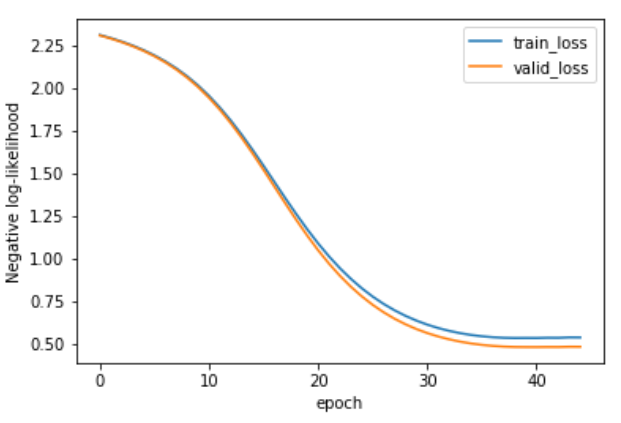
\includegraphics[width=\textwidth]{error_mnist}
		\caption{Erreur}
	\end{subfigure}
	\begin{subfigure}{0.45\textwidth}
		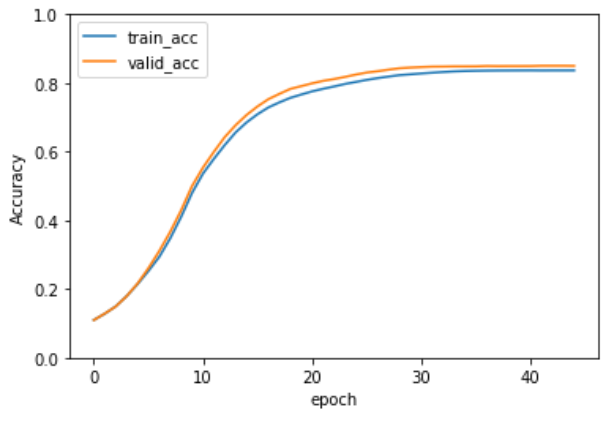
\includegraphics[width=\textwidth]{accuracy_mnist}
		\caption{Précision}
	\end{subfigure}
	\caption{Précision et erreur sur les ensembles d'apprentissage et de validation de MNIST}
\end{figure}

Nous remarquons que l'erreur sur les ensembles d'apprentissage et de validation diminue efficacement au fil des itérations, puis commence à se stabiliser à la fin lorsque on se trouve dans un optimium local.

Nous remarquons que même sans utiliser la régularisation, le modèle ne souffre pas de sur apprentissage, vu que la courbe d'erreur sur l'ensemble de validation ne diverge pas de celle de l'ensemble d'apprentissage (L1 et L2 ont été testées mais les résultats sont presque les mêmes)

Quant à la précision, nous remarquons qu'elle est en train d'augmenter pour les deux ensembles, jusqu'à ce qu'elle se stabilise aux dernières itérations.

\section{Exécution sur la Base de données Cifar 10}
Le programme a été testé aussi sur la base de données $Cifar10$ qui est plus difficile(3072 features au lieu de 784). L'architecture testée est 2 couches cachées avec respectivement 1024 et 512 neurones, fonction d'activation $relu$. Les résultats pour 20 itérations sont les suivants:

\begin{figure}[H]
	\centering
	\begin{subfigure}{0.45\textwidth}
		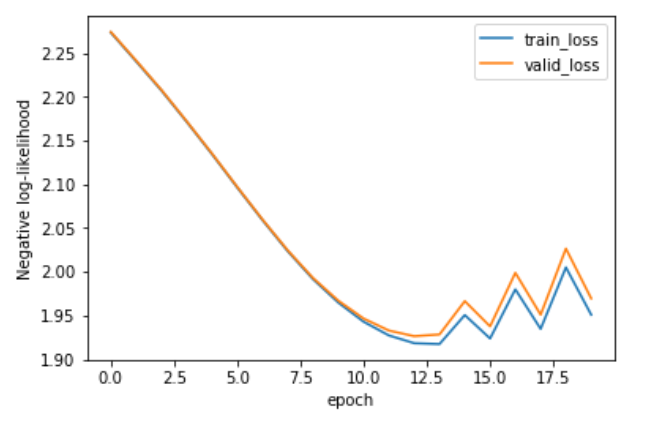
\includegraphics[width=\textwidth]{error_cifar10}
		\caption{Erreur}
	\end{subfigure}
	\begin{subfigure}{0.45\textwidth}
		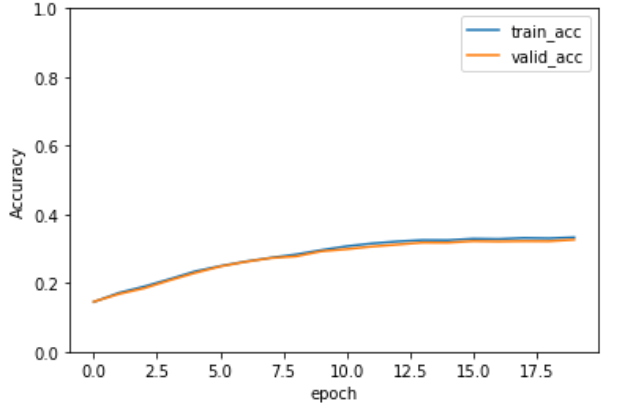
\includegraphics[width=\textwidth]{accuracy_cifar10}
		\caption{Précision}
	\end{subfigure}
	\caption{Précision et erreur sur les ensembles d'apprentissage et de validation de Cifar10}
\end{figure}

Nous remarquons pour la courbe de précision que cette dernière est en train d'augmenter et atteint la valeur 32.92\%. L'erreur est en train de diminuer et elle rencontre des perturbations à la fin des itérations. 

La difficulté d'apprendre une telle base de données est visible. Le temps d'exécution est élevé en le comparant de celui de MNIST, et le réglage de paramètres nécessite plus de tests afin de diminuer l'erreur et augmenter la précision. 

\section{Conclusion}
Ce travail pratique était une occasion pour voir de plus proche le fonctionnement des réseaux de neurones. Ces derniers peuvent changer d'architecture en variant le type du problème, sa difficulté, ses particularités... 

La base de données MNIST représente une tâche de classification simple qui peut être résolue avec un réseau de neurone simple, même sans couches cachées, comme nous l'avons vu dans le travail pratique précédent. En effet, il était possible d'atteindre une précision de 87\% facilement et en un peu de temps.

Les architectures complexes sont plus adaptées aux problèmes complexes, comme Cifar10, qui nécessitent vraiment un réseau profond, c'est la raison pour laquelle on s'est contenté d'une seule couche cachée dans ce travail pour la base de données MNIST.
%%%%%%%%%%%%%%%%%%%%%%%%%%%%%%%%%%%%%%%%%%%%%%%%%%%%%%%%%%%%%
\bibliographystyle{babplain}
\parskip=-1em
%\emptypage{\bibliography{bibliographie}}
\let\section\oldsection % pour éviter que le résumé soient visibles dans le sommaire comme une section
%\include{Resume}
\end{document}
